\documentclass[10pt]{extarticle}
\title{}
\author{Avinash Iyer}
\date{}
\usepackage[shortlabels]{enumitem}

%font setup
%
\usepackage{newpxtext,eulerpx}

%paper setup
\usepackage{geometry}
\geometry{letterpaper, portrait, margin=1in}
\usepackage{fancyhdr}

%symbols
\usepackage{amsmath}
\usepackage{mathtools}
\usepackage{amssymb}
\usepackage{hyperref}
\usepackage{gensymb}

\usepackage[T1]{fontenc}
\usepackage[utf8]{inputenc}

%chemistry stuff
\usepackage[version=4]{mhchem}
\usepackage{chemfig}

%plotting
\usepackage{pgfplots}
\usepackage{tikz}
\tikzset{middleweight/.style={pos = 0.5, fill=white}}
\tikzset{weight/.style={pos = 0.5, fill = white}}
\tikzset{lateweight/.style={pos = 0.75, fill = white}}
\tikzset{earlyweight/.style={pos = 0.25, fill=white}}

%\usepackage{natbib}

%graphics stuff
\usepackage{graphicx}
\graphicspath{ {./images/} }

%code stuff
%when using minted, make sure to add the -shell-escape flag
%you can use lstlisting if you don't want to use minted
%\usepackage{minted}
%\usemintedstyle{pastie}
%\newminted[javacode]{java}{frame=lines,framesep=2mm,linenos=true,fontsize=\footnotesize,tabsize=3,autogobble,}
%\newminted[cppcode]{cpp}{frame=lines,framesep=2mm,linenos=true,fontsize=\footnotesize,tabsize=3,autogobble,}

\usepackage{listings}
\usepackage{color}
\definecolor{dkgreen}{rgb}{0,0.6,0}
\definecolor{gray}{rgb}{0.5,0.5,0.5}
\definecolor{mauve}{rgb}{0.58,0,0.82}

\lstset{frame=tb,
	language=Java,
	aboveskip=3mm,
	belowskip=3mm,
	showstringspaces=false,
	columns=flexible,
	basicstyle={\small\ttfamily},
	numbers=none,
	numberstyle=\tiny\color{gray},
	keywordstyle=\color{blue},
	commentstyle=\color{dkgreen},
	stringstyle=\color{mauve},
	breaklines=true,
	breakatwhitespace=true,
	tabsize=3
}
% text + color boxes
\usepackage{tcolorbox}
\tcbuselibrary{breakable}
\newtcolorbox{problem}[1]{colback = white, title = {#1}, breakable}
\newtcolorbox{solution}{colback = white, colframe = black!75!white, title = Solution, breakable}
%including PDFs
\usepackage{pdfpages}
\setlength{\parindent}{0pt}

\pagestyle{fancy}
\fancyhf{}
\rhead{Avinash Iyer}
\lhead{Homework Section 3.1, Individual}
\begin{document}
  \begin{problem}{3.1.1}
    Find a maximum matching in each graph below. Prove that it is a maximum matching by exhibiting an optimal solution to the dual problem (minimum vertex cover). Explain why this proves that the matching is optimal.
    \begin{center}
      Graph 1:\\
      \vspace{10pt}
      \begin{tikzpicture}
        \filldraw (0,0) circle (2pt)
              (1,0) circle (2pt)
              (2,0) circle (2pt)
              (3,0) circle (2pt)
              (4,0) circle (2pt)
              (0,1) circle (2pt)
              (1,1) circle (2pt)
              (2,1) circle (2pt)
              (3,1) circle (2pt);
        \draw (0,0) -- (2,1);
        \draw (1,0) -- (2,1);
        \draw (2,1) -- (2,0);
        \draw (1,0) -- (3,1);
        \draw (3,1) -- (2,0);
        \draw (3,0) -- (3,1);
        \draw (3,1) -- (4,0);
        \draw (0,1) -- (2,0);
        \draw (1,1) -- (2,0);
        \draw (2,1) -- (4,0);
      \end{tikzpicture}\\
      \vspace{20pt}
      Graph 2:\\
      \vspace{10pt}
      \begin{tikzpicture}
        \filldraw (0,0) circle (2pt)
                  (1,0) circle (2pt)
                  (2,0) circle (2pt)
                  (3,0) circle (2pt)
                  (4,0) circle (2pt);
        \filldraw (0,1) circle (2pt)
                  (1,1) circle (2pt)
                  (2,1) circle (2pt)
                  (3,1) circle (2pt)
                  (4,1) circle (2pt);
        \draw (0,1) -- (1,0);
        \draw (0,1) -- (2,0);
        \draw (1,1) -- (2,0);
        \draw (2,1) -- (1,0);
        \draw (3,1) -- (0,0);
        \draw (3,1) -- (2,0);
        \draw (3,1) -- (3,0);
        \draw (3,1) -- (4,0);
        \draw (4,1) -- (1,0);
        \draw (4,1) -- (2,0);
      \end{tikzpicture}\\
      \vspace{20pt}
      Graph 3:\\
      \vspace{10pt}
      \begin{tikzpicture}
        \filldraw (0,0) circle (2pt)
                  (1,0) circle (2pt)
                  (2,0) circle (2pt)
                  (3,0) circle (2pt)
                  (4,0) circle (2pt);
        \filldraw (0,1) circle (2pt)
                  (1,1) circle (2pt)
                  (2,1) circle (2pt)
                  (3,1) circle (2pt)
                  (4,1) circle (2pt);

        \draw (0,1) -- (1,0);
        \draw (0,1) -- (3,0);

        \draw (1,1) -- (0,0);
        \draw (1,1) -- (1,0);
        \draw (1,1) -- (2,0);
        \draw (1,1) -- (3,0);

        \draw (2,1) -- (1,0);
        \draw (2,1) -- (3,0);

        \draw (3,1) -- (0,0);
        \draw (3,1) -- (1,0);
        \draw (3,1) -- (3,0);
        \draw (3,1) -- (4,0);

        \draw (4,1) -- (1,0);
        \draw (4,1) -- (3,0);
      \end{tikzpicture}
    \end{center}
    \tcblower
    \begin{center}
      Graph 1:\\
      \vspace{10pt}
      \begin{tikzpicture}
        \filldraw (0,0) circle (2pt)
              (1,0) circle (2pt)
              (2,0) circle (2pt)
              (3,0) circle (2pt)
              (4,0) circle (2pt)
              (0,1) circle (2pt)
              (1,1) circle (2pt)
              (2,1) circle (2pt)
              (3,1) circle (2pt);
        \draw[very thick] (0,0) -- (2,1);
        \draw (1,0) -- (2,1);
        \draw (2,1) -- (2,0);
        \draw (1,0) -- (3,1);
        \draw (3,1) -- (2,0);
        \draw[very thick] (3,0) -- (3,1);
        \draw (3,1) -- (4,0);
        \draw[very thick] (0,1) -- (2,0);
        \draw (1,1) -- (2,0);
        \draw (2,1) -- (4,0);
      \end{tikzpicture}\\
      \vspace{10pt}
      \begin{tikzpicture}
        \filldraw (0,0) circle (2pt)
              (1,0) circle (2pt)
              (2,0) circle (2pt)
              (3,0) circle (2pt)
              (4,0) circle (2pt)
              (0,1) circle (2pt)
              (1,1) circle (2pt)
              (2,1) circle (2pt)
              (3,1) circle (2pt);
        \draw (2,1) circle (4pt)
              (2,0) circle (4pt)
              (3,1) circle (4pt);
        \draw (0,0) -- (2,1);
        \draw (1,0) -- (2,1);
        \draw (2,1) -- (2,0);
        \draw (1,0) -- (3,1);
        \draw (3,1) -- (2,0);
        \draw (3,0) -- (3,1);
        \draw (3,1) -- (4,0);
        \draw (0,1) -- (2,0);
        \draw (1,1) -- (2,0);
        \draw (2,1) -- (4,0);
      \end{tikzpicture}\\
      \vspace{20pt}
      Graph 2: \\
      \vspace{10pt}
      \begin{tikzpicture}
        \filldraw (0,0) circle (2pt)
                  (1,0) circle (2pt)
                  (2,0) circle (2pt)
                  (3,0) circle (2pt)
                  (4,0) circle (2pt);
        \filldraw (0,1) circle (2pt)
                  (1,1) circle (2pt)
                  (2,1) circle (2pt)
                  (3,1) circle (2pt)
                  (4,1) circle (2pt);
        \draw[very thick] (0,1) -- (1,0);
        \draw (0,1) -- (2,0);
        \draw (1,1) -- (2,0);
        \draw (2,1) -- (1,0);
        \draw[very thick] (3,1) -- (0,0);
        \draw (3,1) -- (2,0);
        \draw (3,1) -- (3,0);
        \draw (3,1) -- (4,0);
        \draw (4,1) -- (1,0);
        \draw[very thick] (4,1) -- (2,0);
      \end{tikzpicture}\\
      \vspace{10pt}
      \begin{tikzpicture}
        \filldraw (0,0) circle (2pt)
                  (1,0) circle (2pt)
                  (2,0) circle (2pt)
                  (3,0) circle (2pt)
                  (4,0) circle (2pt);
        \filldraw (0,1) circle (2pt)
                  (1,1) circle (2pt)
                  (2,1) circle (2pt)
                  (3,1) circle (2pt)
                  (4,1) circle (2pt);
        \draw (3,1) circle (4pt)
              (2,0) circle (4pt)
              (1,1) circle (4pt);
        \draw (0,1) -- (1,0);
        \draw (0,1) -- (2,0);
        \draw (1,1) -- (2,0);
        \draw (2,1) -- (1,0);
        \draw (3,1) -- (0,0);
        \draw (3,1) -- (2,0);
        \draw (3,1) -- (3,0);
        \draw (3,1) -- (4,0);
        \draw (4,1) -- (1,0);
        \draw (4,1) -- (2,0);
      \end{tikzpicture}\\
      \vspace{20pt}
      Graph 3:\\
      \vspace{10pt}
      \begin{tikzpicture}
        \filldraw (0,0) circle (2pt)
                  (1,0) circle (2pt)
                  (2,0) circle (2pt)
                  (3,0) circle (2pt)
                  (4,0) circle (2pt);
        \filldraw (0,1) circle (2pt)
                  (1,1) circle (2pt)
                  (2,1) circle (2pt)
                  (3,1) circle (2pt)
                  (4,1) circle (2pt);

        \draw[very thick] (0,1) -- (1,0);
        \draw (0,1) -- (3,0);

        \draw[very thick] (1,1) -- (0,0);
        \draw (1,1) -- (1,0);
        \draw (1,1) -- (2,0);
        \draw (1,1) -- (3,0);

        \draw (2,1) -- (1,0);
        \draw[very thick] (2,1) -- (3,0);

        \draw (3,1) -- (0,0);
        \draw (3,1) -- (1,0);
        \draw (3,1) -- (3,0);
        \draw[very thick] (3,1) -- (4,0);

        \draw (4,1) -- (1,0);
        \draw (4,1) -- (3,0);
      \end{tikzpicture}\\
      \vspace{10pt}
      \begin{tikzpicture}
        \filldraw (0,0) circle (2pt)
                  (1,0) circle (2pt)
                  (2,0) circle (2pt)
                  (3,0) circle (2pt)
                  (4,0) circle (2pt);
        \filldraw (0,1) circle (2pt)
                  (1,1) circle (2pt)
                  (2,1) circle (2pt)
                  (3,1) circle (2pt)
                  (4,1) circle (2pt);
        \draw (1,1) circle (4pt)
              (3,0) circle (4pt)
              (1,0) circle (4pt)
              (3,1) circle (4pt);

        \draw (0,1) -- (1,0);
        \draw (0,1) -- (3,0);

        \draw (1,1) -- (0,0);
        \draw (1,1) -- (1,0);
        \draw (1,1) -- (2,0);
        \draw (1,1) -- (3,0);

        \draw (2,1) -- (1,0);
        \draw (2,1) -- (3,0);

        \draw (3,1) -- (0,0);
        \draw (3,1) -- (1,0);
        \draw (3,1) -- (3,0);
        \draw (3,1) -- (4,0);

        \draw (4,1) -- (1,0);
        \draw (4,1) -- (3,0);
      \end{tikzpicture}
    \end{center}
    In all of these cases, we have solved the dual problem and found that the size of the minimum vertex cover is equal to the size of the maximum matching. Because all of these graphs are bipartite, we know that $\alpha'(G) = \beta(G)$.
  \end{problem}
  \begin{problem}{3.1.2}
    Determine the minimum size of a maximal matching in $C_n$.
    \tcblower
    There are two cases of $n$ where we will construct the minimum maximal matching.
    \begin{description}[font=\normalfont\scshape]
      \item[$n$ is odd:] If $n$ is odd, then we create $M$ by selecting one edge, then selecting an edge traversing along $C_n$ by skipping one vertex, then selecting the edge starting from the vertex (if it is not in the matching), then so on and so forth until $M$ cannot be added to. In the case of any odd cycle, this means $|M| = \left\lfloor \frac{n}{2}\right\rfloor$.
      \item[$n$ is even] If $n$ is even, then we create $M$ by selecting an edge and traversing along the cycle by a similar technique (skip one vertex, select an edge starting at the following vertex, etc.) until $M$ cannot be added to any further. This yields a minimum size of $|M| = \frac{n}{2} - 1$, as we can select two vertices to be skipped in any graph.
    \end{description}
  \end{problem}
  \begin{problem}{3.1.5}
    Prove that $\alpha(G) \geq \frac{n(G)}{\Delta(G)+1}$ for every graph $G$.
  \end{problem}
  \begin{problem}{3.1.9}
    Prove that every maximal matching in a graph $G$ has at least $\alpha'(G)/2$ edges.
  \end{problem}
  \begin{problem}{3.1.28}
    Exhibit a perfect matching in the graph below or give a short proof that it has none. 
    \begin{center}
      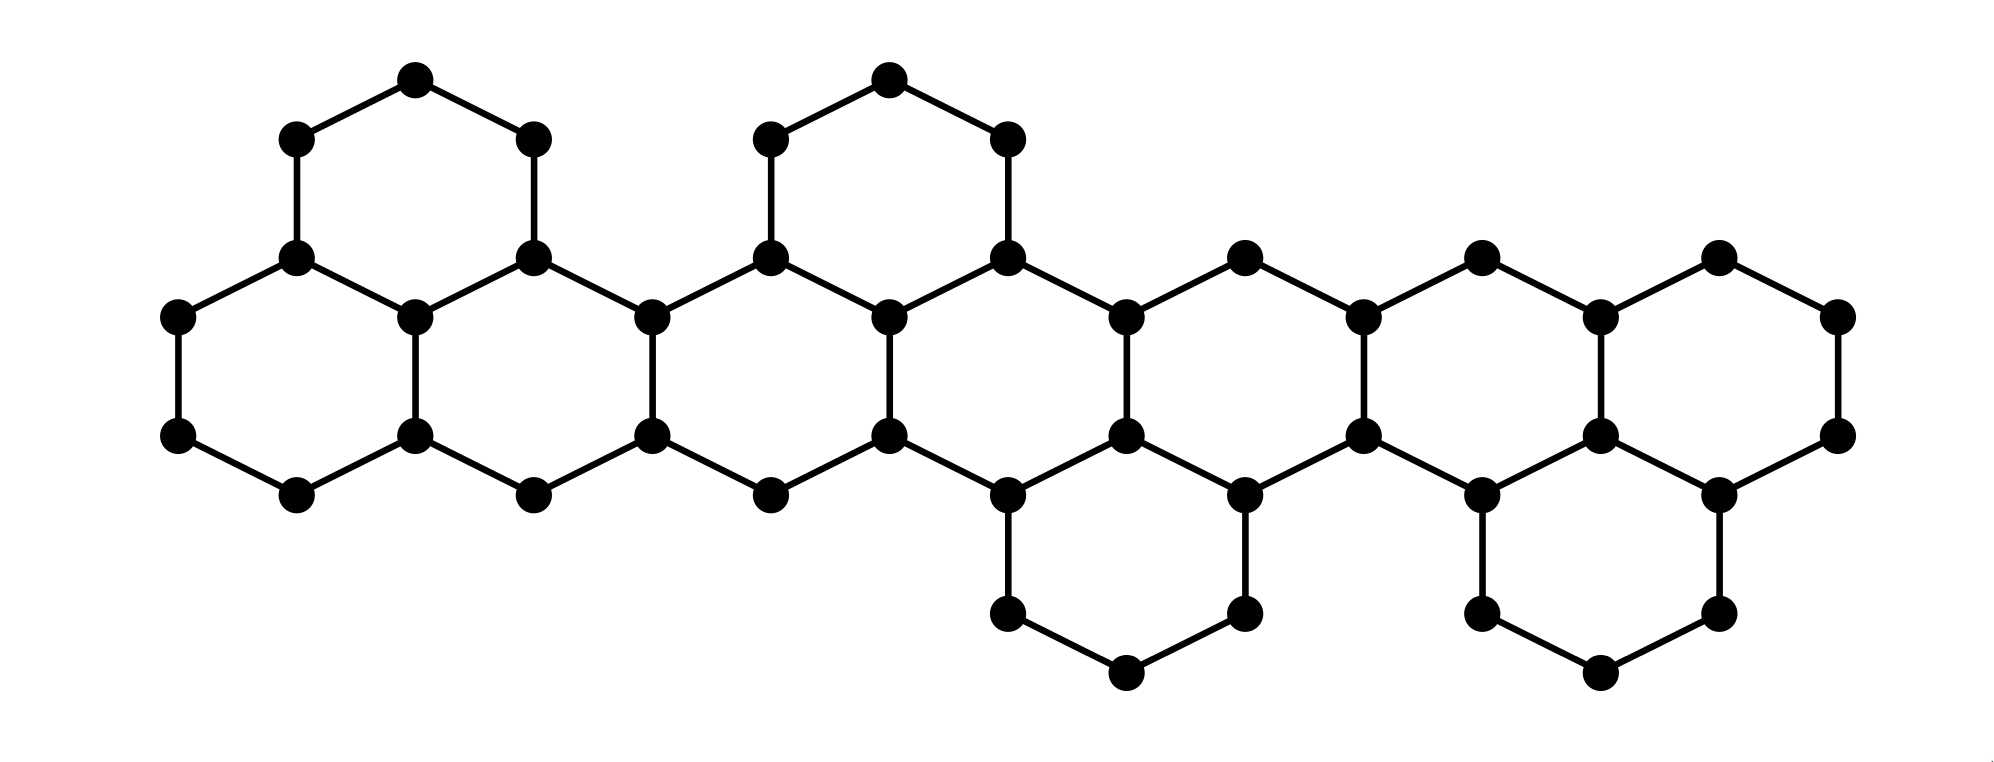
\includegraphics[width=10cm]{3_1_28_question}
    \end{center}
  \end{problem}
\end{document}
